
\chapter{Parity in black-box \textsf{TFNP}} \label{chap:parity-tfnp}

\section{Parity decision trees}

The concept of parity is extensively studied in computer science. In our case, we are interested in exploring parity through the lens of \textit{linear forms modulo 2}, i.e. linear equations defined on $n$ variables over the algebraic field $\F_2$. In this field, each term can either be a 0 or a 1, with the defining characteristic that $1+1 = 0$.

\begin{definition}
 Given $n$ variables $x_1, \ldots, x_n$, we define a \textbf{linear form} as a linear equation over $\F_2$. In general, a linear form can be expressed as $\sum\limits_{i = 1}^n \alpha_i x_i$, where $\alpha_1, \ldots, \alpha_n \in \F_2$
\end{definition}

Intuitively, each sum in a linear form is nothing more than an application of the XOR operator: the linear form $x_1 + x_2$ is equal to 1 if and only if $x_1$ is \textit{different} from $x_2$ (i.e. if $x_1 = 1$ and $x_2 = 0$ or if $x_1 = 0$ and $x_2 = 1$). Additionally, in $\F_2$ the concepts of addition and subtraction are equivalent: since $1+1 = 0$, we easily get that $1 = -1$. Through these properties, parity can be used to determine if two or more objects are equal or not. For example, consider the following system of linear forms:
\[\left \{ \begin{array}{l}
 x_1 + x_2 + x_3 = 1 \\
 x_1 + x_2 + x_4 = 1 \\
 x_1 + x_3 = 1
\end{array} \right .\]

By simplifying the linear system we get that:
\[\left \{ \begin{array}{l}
 x_1 + x_2 + x_3 = 1 \\
 x_1 + x_2 + x_4 = 1 \\
 x_1 + x_3 = 1
\end{array} \right . \longrightarrow
\left \{ \begin{array}{l}
 x_2 = 1\\
 x_1 + 1 + x_4 = 1 \\
 x_1 + x_3 = 1
\end{array} \right . \longrightarrow
\left \{ \begin{array}{l}
 x_2 = 1\\
 x_1 = x_4 \\
 x_1 = 1+x_3
\end{array} \right .\]

which tells us that $x_2 = 1$ and $x_1 = x_4 \neq x_3$ must hold.

\newpage

But what happens if we apply the concept of parity in decision trees? What if, instead of querying variables to know their value, we ask the parity of a set of values by querying linear forms? This idea gives rise to the extended model of \textbf{parity decision trees}.

Instead of being labeled by single variables, the nodes of a parity decision tree (PDT for short) are labeled by a linear form $f$. Each node has two outgoing edges, one labeled by $f = 0$ and the other by $f = 1$. Every path from the root of the PDT to one of its nodes defines a system of linear forms given by all the labels of the edges on the path. In general, given the PDT $T$ and a node $v$, we denote this system with $\Phi_v^T$. Given an assignment $\alpha(x_1, \ldots, x_n)$, the output of a PDT is dictated by the parity queries made by each node.

\begin{figure}[H]
    \centering

    \begin{tikzpicture}[->,>=stealth,shorten >=1pt,auto,node distance=1.75cm, thick,main node/.style={scale=0.9,circle,draw,font=\sffamily\normalsize}]

        \node[ellipse, draw] (1)[] {$x_1+x_2+x_3$};

        \node[ellipse, draw] (2) [below left of=1, xshift=-50, ]{$x_1+x_2$};
        \node[ellipse, draw] (3) [below right of=1, xshift=50, ]{$x_1$};

        \node[ellipse, draw] (4) [below left of=2, xshift=-10, ]{$x_2+x_3$};
        \node[ellipse, draw] (5) [below right of=2, xshift=10, ]{$x_2$};
        \node[ellipse, draw] (6) [below left of=3, ]{$x_2$};
        \node[rectangle, draw] (7) [below right of=3]{$o_7$};

        \node[rectangle, draw] (8) [below left of=4, xshift=10, yshift=-10]{$o_1$};
        \node[rectangle, draw] (9) [below right of=4, xshift=-10, yshift=-10]{$o_2$};
        \node[rectangle, draw] (10) [below left of=5, xshift=10, yshift=-10]{$o_3$};
        \node[rectangle, draw] (11) [below right of=5, xshift=-10, yshift=-10]{$o_4$};
        \node[rectangle, draw] (12) [below left of=6, xshift=10, yshift=-10]{$o_5$};
        \node[rectangle, draw] (13) [below right of=6, xshift=-10, yshift=-10]{$o_6$};

        \path[every node/.style={font=\sffamily\small}]
            (1) edge[swap, color=Green]  node{0} (2)
            (1) edge node{1}(3)

            (2) edge[swap]  node{0} (4)
            (2) edge[color=Green]  node{1}(5)

            (3) edge[swap]  node{0} (6)
            (3) edge  node{1}(7)
                        
            (4) edge[swap]  node{0} (8)
            (4) edge  node{1}(9)

            (5) edge[swap]  node{0} (10)
            (5) edge[color=Green]  node{1}(11)

            (6) edge[swap]  node{0} (12)
            (6) edge  node{1}(13)
            ;
    \end{tikzpicture}

    \caption{An example of a parity decision tree of size 13 and depth 3.}
\end{figure}

In the above example, the green path defines the following system of linear forms:
\[\left \{ \begin{array}{l}
 x_1 + x_2 + x_3 = 0 \\
 x_1 + x_2 = 1 \\
 x_2 = 1
\end{array}\right .\]

which once simplified corresponds to the assignment $x_0 = 0, x_2 = 1, x_3 = 1$. We define the class $\mathsf{FP}^{pdt}$ as the set of $\mathsf{TFNP}^{dt}$ problems that are efficiently solvable by a PDT, where the complexity measures are defined as in normal decision trees.

\begin{definition}
 We define $\mathsf{FP}^{pdt}$ as the set of query search problems $R = (R_n)_{n \in \N}$ for which there exists a polylogarithmic depth PDT $T_n$ such that $T_n(x) = y$ if and only if $(x,y) \in R_n$.
\end{definition}

It's easy to see that $\mathsf{FP}^{dt} \subseteq \mathsf{FP}^{pdt}$ since any decision tree is just a PDT with all the queries defined only on one variable. Any PDT can be converted into a normal decision tree simply by "splitting" each linear query. Given a node $v$ labeled with the linear form $f + x_i$, let $u$ and $w$ be the children of $v$ respectively given by $f + x_i = 0$ and $f+x_i = 1$. Let $T_u$ and $T_w$ be the two subtrees with root $u$ and $w$.

\newpage

\begin{figure}[H]
    \centering

    \begin{tikzpicture}[->,>=stealth,shorten >=1pt,auto,node distance=1.75cm, thick,main node/.style={scale=0.9,circle,draw,font=\sffamily\normalsize}]

        \node[ellipse, draw] (1)[] {$f + x_i$};

        \node[circle, draw] (2) [below left of=1, xshift=-50, ]{};
        \node[circle, draw] (3) [below right of=1, xshift=50, ]{};

        \node[] (2a) [below left of=2, yshift=-40]{};
        \node[] (2b) [below right of=2, yshift=-40]{};
        \node[] (2c) [below of=2]{$T_u$};

        \node[] (3a) [below left of=3, yshift=-40]{};
        \node[] (3b) [below right of=3, yshift=-40]{};
        \node[] (3c) [below of=3]{$T_w$};

        \path[every node/.style={font=\sffamily\small}]
            (1) edge[swap]  node{0} (2)
            (1) edge node{1}(3)
            ;

        \path[every node/.style={font=\sffamily\small}, -]
            (2) edge (2a.center)
            (2) edge (2b.center)
            (2a.center) edge (2b.center)
            ;

        \path[every node/.style={font=\sffamily\small}, -]
            (3) edge (3a.center)
            (3) edge (3b.center)
            (3a.center) edge (3b.center)
            ;
    \end{tikzpicture}

    \caption{The initial subtree of a parity decision tree}
\end{figure}

We replace $v$ with the node $v'$ labeled with the linear form $x_i$ and introduce two new nodes $u', w'$ such that $u'$ is the child of $v'$ when $x_i = 0$ and $w'$ is the child of $v'$ when $x_i = 1$. We label $u'$ with the linear form $f$ and let a copy of $T_u$ be the children of $u'$ when $f = 0$, while a copy of $T_w$ is the children of $u'$ when $f = 1$. Symmetrically, we label $w'$ with the linear form $f$ and let a copy of $T_w$ be the children of $w'$ when $f = 0$, while a copy of $T_u$ is the children of $w'$ when $f = 1$. 

\begin{figure}[H]
    \centering

    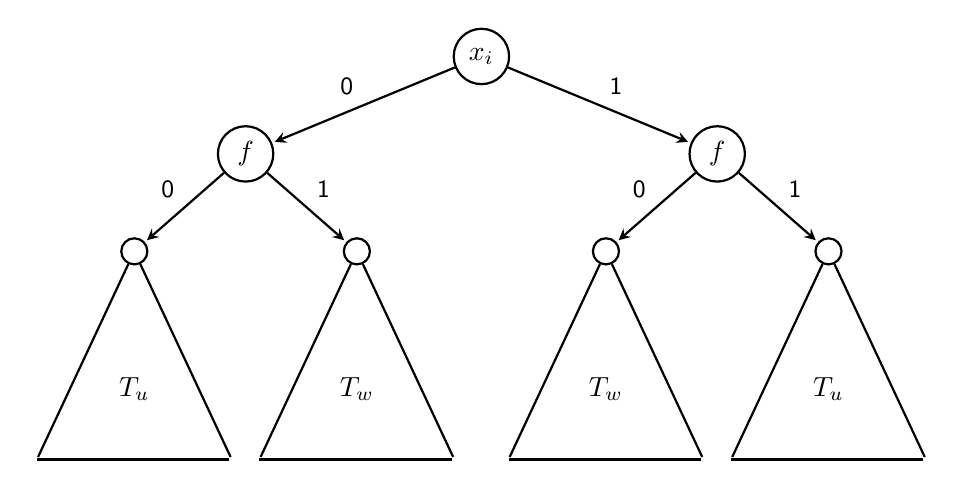
\begin{tikzpicture}[->,>=stealth,shorten >=1pt,auto,node distance=1.75cm, thick,main node/.style={scale=0.9,circle,draw,font=\sffamily\normalsize}]

        \node[circle, draw] (1)[] {$x_i$};

        \node[circle, draw] (2) [below left of=1, xshift=-50, ]{$f$};
        \node[circle, draw] (3) [below right of=1, xshift=50, ]{$f$};

        \node[circle, draw] (2x) [below left of=2, xshift=-5]{};
        \node[circle, draw] (2y) [below right of=2, xshift=5]{};

        \node[circle, draw] (3x) [below left of=3, xshift=-5]{};
        \node[circle, draw] (3y) [below right of=3, xshift=5]{};

        \node[] (2a) [below left of=2x, yshift=-40]{};
        \node[] (2b) [below right of=2x, yshift=-40]{};
        \node[] (2c) [below of=2x]{$T_u$};

        \node[] (3a) [below left of=2y, yshift=-40]{};
        \node[] (3b) [below right of=2y, yshift=-40]{};
        \node[] (3c) [below of=2y]{$T_w$};

        \node[] (4a) [below left of=3x, yshift=-40]{};
        \node[] (4b) [below right of=3x, yshift=-40]{};
        \node[] (4c) [below of=3x]{$T_w$};

        \node[] (5a) [below left of=3y, yshift=-40]{};
        \node[] (5b) [below right of=3y, yshift=-40]{};
        \node[] (5c) [below of=3y]{$T_u$};

        \path[every node/.style={font=\sffamily\small}]
            (1) edge[swap]  node{0} (2)
            (1) edge node{1}(3)

            (2) edge[swap]  node{0} (2x)
            (2) edge node{1}(2y)

            (3) edge[swap]  node{0} (3x)
            (3) edge node{1}(3y)
            ;

        \path[every node/.style={font=\sffamily\small}, -]
            (2x) edge (2a.center)
            (2x) edge (2b.center)
            (2a.center) edge (2b.center)
            ;

        \path[every node/.style={font=\sffamily\small}, -]
            (2y) edge (3a.center)
            (2y) edge (3b.center)
            (3a.center) edge (3b.center)
            ;

        \path[every node/.style={font=\sffamily\small}, -]
            (3x) edge (4a.center)
            (3x) edge (4b.center)
            (4a.center) edge (4b.center)
            ;

        \path[every node/.style={font=\sffamily\small}, -]
            (3y) edge (5a.center)
            (3y) edge (5b.center)
            (5a.center) edge (5b.center)
            ;
    \end{tikzpicture}

    \caption{The subtree after the splitting process}
\end{figure}

By repeating this process until all queries are defined on a single variable, we obtain a decision tree equivalent to the original PDT. This final decision tree has exponential size and polynomial depth, which \textit{may not} be the smallest possible decision tree that solves the search problem solved by the initial PDT. However, we can easily prove that parity decision trees are indeed much stronger than decision trees.

\begin{theorem}
    \label{fp_pdt_not_inside_fp_dt}
    $\mathsf{FP}^{dt} \subsetneq \mathsf{FP}^{pdt}$
\end{theorem}

\begin{proof}
 Consider the search problem of determining the parity of $n$ variables for a given assignment $\alpha$. This problem can be solved by a PDT that makes a single query on all $n$ variables. By applying the splitting process to this tree, we get a decision tree of size $2^n$ and depth $n$. It's easy to see that the resulting decision tree is the smallest possible tree that can solve this search problem.
\end{proof}

\newpage

Since a system of linear forms can have multiple solutions, many assignments could be mapped to the same output. However, some systems could also be unsatisfiable, meaning that the node is unreachable by any assignment. When this happens we say that the node is \textbf{degenerate}.

Like normal decision trees, PDTs can be used to solve the false clause search problem associated with any unsatisfiable CNF. A parity decision tree for a CNF formula $F$ is a PDT defined on the same variables of $F$ where for each leaf $v$ one of the following conditions holds:
\begin{enumerate}[itemsep=0em]
    \item The leaf is \textit{degenerate}
    \item The leaf \textit{refutes} a clause $C$ of $F$, meaning that the system $\Phi_v^T$ is satisfiable and every one of its solutions falsifies $C$
    \item The leaf \textit{satisfies} a clause $C$ of $F$, meaning that the system $\Phi_v^T$ has only one solution and it also satisfies $C$
\end{enumerate}

\begin{figure}[H]
    \centering

    \begin{tikzpicture}[->,>=stealth,shorten >=1pt,auto,node distance=1.75cm, thick,main node/.style={scale=0.9,circle,draw,font=\sffamily\normalsize}]

        \node[ellipse, draw] (1)[] {$x + y$};

        \node[ellipse, draw] (2) [below left of=1, xshift=-20, ]{$x$};
        \node[ellipse, draw] (3) [below right of=1, xshift=20, ]{$x$};

        \node[rectangle, draw] (4) [below left of=2, xshift=10, yshift=-10]{$x \lor y$};
        \node[rectangle, draw] (5) [below right of=2, xshift=-10, yshift=-10]{$\lnot x \lor \lnot y$};
        \node[rectangle, draw] (6) [below left of=3, xshift=10, yshift=-10]{$x \lor \lnot y$};
        \node[rectangle, draw] (7) [below right of=3, xshift=-10, yshift=-10]{$\lnot x \lor y$};

        \path[every node/.style={font=\sffamily\small}]
            (1) edge[swap]  node{0} (2)
            (1) edge node{1}(3)

            (2) edge[swap]  node{0} (4)
            (2) edge[]  node{1}(5)

            (3) edge[swap]  node{0} (6)
            (3) edge  node{1}(7)
                        
            ;
    \end{tikzpicture}

    \caption{A parity decision tree for $(x \lor y) \land (\lnot x \lor \lnot y) \land (\lnot x \lor y) \land (x \lor \lnot y)$}
\end{figure}

We observe that if a node doesn't meet any of the previous conditions then it cannot be a leaf node. Moreover, we also observe that the system associated with the root of any PDT is always satisfiable due to it containing no linear forms. Since we are interested in studying PDTs for refusing unsatisfiable CNF formulas, the third case will never be true for any leaf. However, we still need a way to exclude the first case since an unsatisfiable system cannot be associated with any assignment. Luckily, each degenerate PDT can be conveniently converted into a non-degenerate one through a very simple process \cite{res_lin_2}.

\begin{proposition}
    \label{degenerate}
 Let $F$ be an unsatisfiable CNF formula. If $S_F$ can be solved with a degenerate PDT of size $s$ and depth $d$, it can also be solved with a non-degenerate PDT of size at most $s$ and depth at most $d$.
\end{proposition}

\begin{proof}
    
 Let $T$ be a degenerate PDT of size $s$ and depth $d$ that solves $S_F$. Let $U$ be the set of degenerate nodes of $T$. Notice that since $\Phi_r^T$ is empty, thus always satisfiable, we know that $r \notin U$. Consider the node $u \in U$ with the minimal distance from the root $r$. Since $u$ is not the root of $T$, there must be two vertices $p$ and $s$ such that $p$ is the parent of $u$ and $s$ is the sibling of $u$.

 We notice that $\Phi_s^T$ must be satisfiable: if we assume that this is not true then both $\Phi_s^T$ and $\Phi_u^T$ would be unsatisfiable, which can be true only if $\Phi_p^T$ is also unsatisfiable, but we chose $w$ as the node in $U$ with minimal distance. Since $\Phi_s^T$ is satisfiable, the label $f = \alpha$ on the edge $(p,s)$ must be already contained inside the system $\Phi_p^T$, meaning that each assignment that satisfies $\Phi_p^T$ also satisfies $\Phi_s^T$.

 We construct a new PDT $T'$ by removing the subtree $T_u$ with root $u$ from the initial PDT $T$ and by contracting the edge $(p,s)$, merging the two nodes $p$ and $s$ into a single node $v$. In other words, the subtree $T_u$ gets removed and the children of $s$ become the new children of $p$. Each assignment that satisfies $\Phi_p^T$ also satisfies $\Phi_v^{T'}$, concluding that $T'$ also solves $S_F$. By repeating the process until $U$ is empty, we get a non-degenerate PDT that solves $S_F$ of size at most $s$ and depth at most $d$.
\end{proof}

\section{Linear Resolution over $\F_2$}

Once we have defined the class $\mathsf{FP}^{pdt}$, we are interested in finding a proof system that characterizes it. Consider a system $\Phi$ of linear forms defined on $\F_2$. This system can be viewed as the conjunction of the linear forms that it describes:
\[\left \{ \begin{array}{c}
 f_1 = \alpha_1 \\
 f_2 = \alpha_2 \\
    \vdots \\
 f_k = \alpha_k
\end{array}\right . \iff (f_1 = \alpha_1) \land (f_2 = \alpha_2) \land \ldots \land (f_k = \alpha_k)\]

We can rewrite these conjunctions as a negation of a disjunction:
\[\bigwedge_{i = 1}^k (f_i = \alpha_i) \iff \lnot \bigvee_{i = 1}^k \lnot (f_i = \alpha_i) \iff \lnot \bigvee_{i = 1}^k (f_i = 1 + \alpha_i)\]

which implies that the negation of the system is equivalent to a set of disjunctions:
\[\lnot \bigwedge_{i = 0}^k (f_1 = \alpha_1) \iff \bigvee_{i = 0}^k (f_1 = 1 + \alpha_1)\]

We define such a set of disjunctions as a \textbf{linear clause}. More generally, a \textit{linear CNF formula} over $\F_n$ is a conjunction of linear clauses defined on $\F_n$.

\begin{definition}
 A linear CNF formula is a conjunction of $m$ disjunctions of linear equations over $\F_n$.
    \[\bigwedge_{i = 1}^m \bigvee_{j = 1}^{k_i} (f_j = \alpha_j)\]
\end{definition}

Linear CNF formulas can assume a complex structure such as the following:
\[((x_1+x_2 = 0) \lor (x_1 = 1)) \land ((x_2 + x_3 + x_4 = 3) \lor (x_2 + x_4 = 0))\]

\newpage

We define \textbf{Linear Resolution over $\F_n$} (or $\mathsf{ResLin(\F_n)}$), an extension of standard Resolution (see \Cref{chap:bb-tfnp}) based on the following two rules:
\begin{enumerate}
    \item \textit{Resolution rule}: given two linear clauses $(f = 0) \lor C$ and $(f = 1) \lor D$ defined on $\F_n$, we can derive the linear clause $C \lor D$
    \item \textit{Weakening rule}: given a linear clause $C$, we can derive any linear clause $D$ such that $C \implies D$.
\end{enumerate}

Like in normal Resolution, in $\mathsf{ResLin(\F_n)}$ any derivation of a linear clause $C$ from a linear CNF $F$ is a sequence of linear clauses that ends with $C$, where every clause is either an axiom of $F$ or it can be derived from previous clauses through one of the two derivation rules. A linear CNF is unsatisfiable if and only if the empty linear clause can be derived from it. 

Any standard CNF formula can be described as a linear CNF formula over $\F_2$ simply by treating each clause as a disjunction of linear forms made of a single term. For example, the CNF $(x_1 \lor \lnot{x_2}) \land (\lnot{x_3} + x_1)$ can be written as the following linear CNF formula:
\[((x_1 = 1) \lor (x_2 = 0)) \land ((x_3 = 0) \lor (x_1 = 1))\]

We call this the \textit{linear encoding} of a CNF. From now on, we will restrict our interests to Linear Resolution over $\F_2$, also called \textit{parity Resolution} (or $\mathsf{Res}_\oplus$).

The weakening rule makes this proof system powerful thanks to how semantical implications can be used as "shortcuts". For example, consider the following linear CNF:
\[(x = 1) \land (x+y = 1) \land ((x = 0) \lor (y = 1))\]

By rewriting the last linear clause as a negation of a conjunction, we notice that:
\[(x = 0) \lor (y = 1) \equiv \lnot ((x = 1) \land (y = 0))\]

By simple substitution, we get that:
\[\lnot ((x = 1) \land (y = 0)) \implies  \lnot ((x = 1) \land (x+y = 1))\]

which is equivalent to:
\[\lnot ((x = 1) \land (x+y = 1)) \equiv (x = 0) \lor (x+y = 0)\]

concluding that $(x = 0) \lor (y = 1) \models (x = 0) \lor (x+y = 0)$. Proceeding with the resolution rule, we get the following Tree-like refutation.
\begin{figure}[H]
    \centering
    
    \begin{tikzpicture}[-,>=stealth,shorten >=1pt,auto,node distance=2.25cm, thick,main node/.style={scale=0.9,circle,draw,font=\sffamily\normalsize}]
    
        \node (1) []{$\bot$};
        
        \node (3) [above right of=1]{$(x = 0)$};
    
        \node (6) [above right of=3]{$(x=0) \lor (x+y = 0)$};
        
        \node (8) [above of=6]{$(x = 0) \lor (y = 1)$};
    
        \node (14) at ($(8)+(-4,0)$){$(x+y=1)$};
        \node (15) [left of=14]{$(x=1)$};
    
        \path[every node/.style={font=\sffamily\small}]
            (14) edge (3)
            (15) edge (1)
               
            (8) edge (6)
               
            (6) edge (3)
               
            (3) edge (1)
            ;
    \end{tikzpicture}

    \caption{$\mathsf{TreeRes}_\oplus$-proof of the previous linear CNF formula}
    \label{treelike_proof}
\end{figure}

It was shown that the weakening rule can be simulated through these simple three rules \cite{res_lin_2}:
\begin{enumerate}
    \item \textit{Simplification rule}: given a linear clause $C \lor (0 = 1)$, we can derive the linear clause $C$
    \item \textit{Syntactic weakening}: given a linear clause $C$, we can derive the linear clause $C \lor (f = \alpha)$
    \item \textit{Addition rule}: given a linear clause $C \lor (f = \alpha) \lor (g = \beta)$, we can derive the linear clause $C \lor (f = \alpha) \lor (g = \beta)$
\end{enumerate}

\begin{proposition}
 Any clause obtainable through the weakening rule can also be obtained through a sequence of applications of the previous three rules and vice versa.
\end{proposition}

This result makes working with the weakening rule easier: any clause $D$ derived through $k$ applications of these three rules starting from a clause $C$ is automatically a weakening of $C$, implying that we can replace those $k$ applications with one single use of the weakening rule.

\section{Characterization of $\textsf{FP}^{pdt}$ through $\mathsf{TreeRes}_\oplus$}

$\mathsf{TreeRes}_\oplus$ proofs and parity decision trees can be viewed as two sides of the same coin. Any tree-like $\ResP$ refutation of a linear CNF $F$ can be used to construct an (almost) equivalent PDT that solves $S_F$ and vice versa \cite{res_lin_2}.

\begin{lemma}
    \label{resp_to_pdt}
 Let $F$ be a linear CNF formula. If there is a $\mathsf{TreeRes}_\oplus$ refutation of $F$ with size $s$ and depth $d$, there also is a PDT of size at most $s$ and depth at most $d$ that solves $S_F$.
\end{lemma}

\begin{proof}
 Let $T$ be the proof tree that refutes $F$. We label each edge of $T$ whose associated clauses involve a resolution rule, while all the other weakening edges remain unlabeled. In particular, if a resolution rule is applied to the clauses $(f = 0) \lor D_1$ and $(f = 1) \lor D_2$ obtaining the clause $D_1 \lor D_2$, we label the edge from the first to the third with $f = 1$, while the other edge is labeled with $f = 0$.

 By induction on the depth of a vertex of $T$, we show that the clause written in $v$ contradicts the system $\Phi_v^T$. The root node contains the empty clause and is labeled by an empty system, making the statement trivially true. Assume now that the statement holds for a generic node $v$. We have to show that the hypothesis also holds for its children $u$ and $w$.

 Suppose that $v$ is the result of a resolution rule application, where $D_1 \lor D_2$ is the clause inside $v$. Assume that $u$ is the node that contains $(f = 0) \lor D_1$ while $w$ contains $(f = 1) \lor D_2$. By inductive hypothesis, we know that $D_1 \lor D_2$ contradicts the system $\Phi_v^T$ and equivalently that the system $\lnot (\lnot D_1 \land \lnot D_2)$ contradicts $\Phi_v^T$. This means that se of equalities in $D_1$ contradict $\Phi_v^T$. Moreover, we know that $\Phi_u^T = \Phi_v^T \land (f = 1)$, concluding that $(f = 0) \lor D_1$ contradicts $\Phi_u^T$. Likewise, we can show that $(f = 1) \lor D_2$ contradicts $\Phi_w^T$.
    
 Suppose now that $v$ is the result of a weakening rule, where $u$ is the only child. Since $(v,u)$ is unlabeled, we get that $\Phi_v^T = \Phi_u^T$. Furthermore, since $v$ is the result of a weakening applied to $u$, we know that the clause in $u$ semantically implies the clause in $v$, but by inductive hypothesis we know that the clause in $v$ contradicts the system $\Phi_v^T$, meaning that $u$ must also contradict the system $\Phi_v^T = \Phi_u^T$. Finally, if $v$ is a leaf then the statement is trivially true since it refutes a clause of $F$.

 By contracting all the unlabeled edges given by the weakening rules, we get a parity decision tree that solves $S_F$. Due to this final step, the size of the PDT is at most $s$ and its depth is at most $d$. 
\end{proof}

\begin{figure}[H]
    \centering

    \begin{tikzpicture}[->,>=stealth,shorten >=1pt,auto,node distance=1.75cm, thick,main node/.style={scale=0.9,circle,draw,font=\sffamily\normalsize}]

        \node[circle, draw] (1)[] {$x$};

        \node[rectangle, draw] (2) [below left of=1, xshift=-20, ]{$x = 1$};
        \node[ellipse, draw] (3) [below right of=1, xshift=20, ]{$x+y$};

        \node[rectangle, draw] (4) [below left of=3, xshift=-20, yshift=-10]{$x+y = 1$};
        \node[rectangle, draw] (5) [below right of=3, xshift=20, yshift=-10]{$(x = 0) \lor (y = 1)$};

        \path[every node/.style={font=\sffamily\small}]
            (1) edge[swap]  node{0} (2)
            (1) edge node{1}(3)

            (3) edge[swap]  node{0} (4)
            (3) edge[]  node{1}(5)            
            ;
    \end{tikzpicture}

    \caption{The PDT obtained from the proof shown in \Cref{treelike_proof}}
    \label{pdt_cnf}
\end{figure}

\begin{lemma}
    \label{pdt_to_resp}
 Let $F$ be a linear CNF formula. If there is a PDT of size $s$ and depth $d$ that solves $S_F$, there also is a $\mathsf{TreeRes}_\oplus$ refutation of $F$ with size at most $2s$, depth at most $d+1$ and the weakening rule applied only to the axioms.
\end{lemma}

\begin{proof}
 Let $T$ be a PDT of size $s$ and depth $d$ that solved $S_F$. By \Cref{degenerate}, we assume that $T$ is non-degenerate. We label every node $v$ of $T$ with the negation of its associated linear system. In other words, every node $v$ is labeled with the linear clause $\lnot \Phi_v^T$. Every node is the result of the resolution rule being applied to its children, where the root node is the empty clause.

 Since $T$ is a PDT that solves $S_F$, each leaf refutes a linear clause of $F$. Hence, for each leaf $u$ we have that $\Phi_{u}^T \implies \lnot C$ for some linear clause $C$ of $F$, which equivalently means that $C \implies \lnot \Phi_u^T$, concluding that the linear clause of each leaf is actually the weakening of a clause of $F$. Then, for each leaf $u$ we can add a new neighbor node $w$ and label it with the clause $C$, where the edge $(w,u)$ becomes an application of the weakening rule. This process increases the depth of the tree by 1 and increases the size by at most $s$.
\end{proof}

\begin{figure}[H]
    \centering
    
    \begin{tikzpicture}[-,>=stealth,shorten >=1pt,auto,node distance=2.25cm, thick,main node/.style={scale=0.9,circle,draw,font=\sffamily\normalsize}]
    
        \node (1) []{$\bot$};
        
        \node (3) [above right of=1, xshift = 50]{$(x = 0)$};
    
        \node (4) [above left of=3, xshift = -20]{$(x=0) \lor (x+y = 1)$};

        \node (6) [above right of=3, xshift = 20]{$(x=0) \lor (x+y = 0)$};

        
        \node (8) [above of=6]{$(x = 0) \lor (y = 1)$};
    
        \node (14) [above of = 4]{$(x+y=1)$};
        \node (15) [left of=14, xshift = -50]{$(x=1)$};
    
        \path[every node/.style={font=\sffamily\small}]
            (14) edge (4)
            (15) edge (1)
               
            (8) edge (6)
               
            (4) edge (3)
            (6) edge (3)
               
            (3) edge (1)
            ;
    \end{tikzpicture}

    \caption{$\mathsf{TreeRes}_\oplus$-proof obtained from the PDT shown in \Cref{pdt_cnf}}
\end{figure}

We conclude that problems efficiently solvable parity decision trees are indeed characterized by Tree-like Linear Resolution over $\F_2$.

\begin{theorem}
    \label{fp_dt_inside_fp_pdt}
    $\mathsf{FP}^{pdt}(S_F) = \Theta(\mathsf{TreeRes}_\oplus(F))$
\end{theorem}

After defining the class $\mathsf{FP}^{pdt}$ and proving that $\mathsf{TreeRes}_\oplus$ characterizes it, we're interested in studying where this class lies in the \textsf{TFNP}$^{dt}$ hierarchy. It's a well-known fact that was shown that $\mathsf{TreeRes}_\oplus$ can efficiently simulate $\mathsf{TreeRes}$ but the reverse doesn't hold due to the hardness of simulating weakening rules. This result also follows more naturally from our results since $\mathsf{FP}^{dt} \subsetneq \mathsf{FP}^{pdt}$. Parity makes PDTs stronger than decision trees, but how much stronger?

We know that Tree-like Linear Resolution over $\F_2$ is based on linear forms defined on $\F_2$. Since Nullstellensatz over $\F_2$ also works with polynomials over $\F_2$, our intuition was to show that these two proof systems are somehow related to one another.

Initially, our first hypothesis was that $\mathsf{TreeRes}_\oplus$ is a very powerful tool even capable of efficiently simulating $\mathrm{\F_2\text{-}NS}$. We tried to prove this result by showing that $\mathsf{PPA}^{dt} \subseteq \mathsf{FP}^{pdt}$, which appeared to be out of reach. In a seminal paper \cite{res_lin_2}, Itsykson and Sokolov discussed how $\mathsf{TreeRes}_\oplus$ cannot efficiently simulate regular Resolution (or $\mathsf{RegRes}$), a restricted proof system derived from Resolution. Due to any regular Resolution proof also being a Resolution proof, this result also implies that $\mathsf{TreeRes}_\oplus$ cannot efficiently simulate $\mathsf{Res}$. Thanks to \Cref{equiv_proof} and the fact that $\mathrm{PLS}^{dt}(S_F) = \Theta(\mathsf{Res}(F))$, we conclude the following black-box separation.

\begin{corollary}
    \label{pls_not_inside_fp_pdt}
    $\mathsf{PLS}^{dt} \not\subseteq \mathsf{FP}^{pdt}$
\end{corollary}

This rings a bell: looks like PDTs aren't actually that strong. We quickly shifted our perspective on our previous study on relationships with Nullstellensatz, trying to show that the simulation holds in the other direction. Indeed, we were capable of proving that any $\mathsf{TreeRes}_\oplus$ can be converted into a small $\mathrm{\F_2\text{-}Nullstellensatz}$ proof, providing us a \textbf{black-box inclusion} for our new class.

\section{Nullstellensatz}

In 1893, the mathematician Hilbert proved a theorem that established the basis of algebraic geometry, a field that studies the relations between algebra and geometry. This theorem is now known as Hilbert's \textbf{Nullstellensatz} (german for \textit{zero-locus theorem}).

The \textit{weak Nullstellensatz}, a corollary of the stronger theorem, states that given $m$ polynomials $p_1, \ldots, p_m$ defined on $F[x_1, \ldots, x_n]$, where $\F$ is a generic algebraic field, the system $p_1(x) = p_2(x) = \ldots = p_m(x) = 0$ is unsolvable if and only if there are $m$ polynomials $g_1, \ldots, g_m$ defined on $F[x_1, \ldots, x_n]$ such that $\sum_{i=1}^m g_ip_i = 1$.

This weaker version of the theorem has been used to define an \textit{algebraic} proof system, that being a proof system based on polynomial algebra. Intuitively, these proof systems are based on the idea of showing that a set of polynomials $p_1, \ldots, p_m$, called \textit{axioms}, doesn't share a common root, which serves as a proof for the polynomials. In this case, a Nullstellensatz proof is given by the set of polynomials $g_1, \ldots, g_m$ through which we get that $\sum_{i=1}^m g_ip_i = 1$  \cite{ns_definitions}. 

Any CNF formula can be translated to an \textit{algebraic encoding}, a set of polynomials $p_1, \ldots, p_m$ for which the CNF formula is unsatisfiable if and only if there is a Nullstellensatz proof for $p_1, \ldots, p_m$. Given the clause $C = \bigvee_{i = 1}^k x_i \lor \bigvee_{j = 1}^h \lnot y_j$, the algebraic encoding of $C$, written as $p_C$, is given by $p_C := \prod_{i = 1}^{k} x_i \cdot \prod_{j = 1}^h (1- y_j)$.

The algebraic encoding of a CNF formula $F = C_1 \land \ldots \land C_m$ is given by the set of polynomial equations $p_F = \{p_{C_1} = 0, \ldots, p_{C_m} = 0, x_1^2-x_1 = 0, \ldots, x_n^2-x_n = 0\}$. These last polynomials are necessary to impose that the values of $x_1, \ldots, x_n$ are either a 0 or a 1. A Nullstellensatz \textit{refutation} for $F$ is given by the polynomials $g_1, \ldots, g_m, h_1, \ldots, h_n$ such that:
\[\sum_{i = 1}^m g_ip_{C_i} + \sum_{j = 1}^m h_j(x_j^2-x_j) = 1\]

To clear things up, we notice that through this formulation the concept of truthfulness is \textbf{inverted}: the boolean values $0$ and $1$ respectively correspond to the algebraic values $1$ and $0$. For example, the boolean clause $C$ evaluates to 1 when at least a literal inside it evaluates to 1, while an algebraic clause evaluates to 0 when at least a literal inside it evaluates to 0. Likewise, in order for the CNF $F$ to be satisfied by an assignment $x$ each clause must evaluate to 1, while in Nullstellensatz the polynomials inside $p_F$ must all evaluate to 0. 

\begin{figure}[H]
    \centering
    \begin{tabular}{r c l}
 0 & $\longleftrightarrow$ & 1 \\
 1 & $\longleftrightarrow$ & 0 \\
        $x_i$ & $\longleftrightarrow$ & $x_i$ \\
        $\lnot x_i$ & $\longleftrightarrow$ & $1-x_i$ \\
        $C \lor D$ & $\longleftrightarrow$ & $C \cdot D$ \\
        $C \land D$ & $\longleftrightarrow$ & $C + D$ \\
    \end{tabular}

    \caption{Mappings from boolean encoding to algebraic encoding}
\end{figure}

When a polynomial $q$ can be derived from a set of axioms $P$, we write $P \stackrel{\mathsf{NS}}{\vdash} q$. If $F$ is a CNF formula and $P \stackrel{\mathsf{NS}}{\vdash} 1$ then we get a Nullstellensatz refutation.

Consider the following CNF formula:
\[x_1 \land (\lnot x_1 \lor x_2) \land (\lnot x_2 \lor x_3) \land (\lnot x_3 \lor x_4)\land x_4\]
The algebraic encoding is given by $p_1 = x_1$, $p_i = (1-x_{i-1})x_i$ when $2 \leq i \leq 4$ and $p_5 = 1-x_4$. To refute this CNF, we must find the polynomials $g_1, \ldots, g_5, h_1, \ldots, h_4$ through which
\[\sum_{i = 1}^5 g_ip_{i} + \sum_{j = 1}^4 h_j(x_j^2-x_j) = 1\]

To simplify things, we let $h_1, \ldots, h_4 = 0$ in order to have $\sum_{j = 1}^4 h_j(x_j^2-x_j) = 0$.

Let $g_1, \ldots, g_5$ be equal to:
\[\begin{split}
 g_1 &= x_2x_3x_4 \\
 g_2 &= x_3x_4 \\
 g_3 &= x_4 \\
 g_4 &= 1 \\
 g_5 &= 1 \\
\end{split}\]

We easily get that:
\[\begin{split}
    \sum_{i = 1}^5 g_ip_{i}&= x_1x_2x_3x_4 + (1-x_1)x_2x_3x_4 + (1-x_2)x_3x_4 + (1-x_3)x_4 + (1-x_4)\\
    &= x_2x_3x_4 + (1-x_2)x_3x_4 + (1-x_3)x_4 + (1-x_4)\\
    &= x_3x_4 + (1-x_3)x_4 + (1-x_4)\\
    &= x_4 + (1-x_4)\\
    &= 1\\
\end{split}\]

concluding that $P_F \stackrel{\mathsf{NS}}{\vdash} 1$ and thus proving that the CNF is unsatisfiable. In Nullstellensatz, the \textit{size} of a proof is the total number of monomials of the polynomials that make the proof, i.e. the total number of terms in the sum once fully expanded without simplifying any addition (or subtraction). The \textit{degree} of the proof is the maximum degree of any polynomial $g_ip_i$ or $h_j(x^j+x_j)$. For example, the polynomial $(1-x_1)(1-x_2)x_2x_3$ has size 4 and degree 4 since $(1-x_1)(1-x_2)x_2x_3 = x_2x_3 - x_2^2x_3 - x_1x_2x_3 + x_1x_2^2x_3$. The previous proof example has size $1+2+2+2+2 = 9$ and degree $4$.

Nullstellensatz's degree measure vaguely resembles Resolution's width measure. For example, the algebraic encoding of a CNF clause $C$ of width $w$ clearly has degree $w$. Moreover, it's easy to see that a degree upper bound $d$ for the Nullstellensatz refutation of a CNF formula defined on $n$ variables implies a size upper bound of $O(n^{O(d)})$. This result enables us to restrict our interest to the degree of the proof.

\begin{proposition}
 Given a CNF formula $F$ defined on $n$ variables, if $P_F \stackrel{\mathsf{NS}}{\vdash} 1$ with degree $O(d)$ then the size of the proof is $n^{O(d)}$.
\end{proposition}

A common result shows that in Nullstellensatz proofs we can assume that polynomials are \textit{multilinear} (short for \textit{multivariate and linear}), meaning that each variable of each term has algebraic multiplicity equal to at most. For example, the polynomial $xy+yz$ is multilinear, while $x^2y$ isn't. This assumption affects the degree of the proof only by a constant factor, which is negligible, allowing us to work easier.


\unsure{Maybe add a small part on how $\F_2$-$\mathsf{NS}$ equals $\mathsf{PPA}^{dt}$}


\section{From $\mathrm{TreeRes}_\oplus$ to $\F_2$-Nullstellensatz}

We prove that Nullstellensatz over $\F_2$ is capable of efficiently simulating $\mathrm{TreeRes}_\oplus$. Given the linear clause $C = \bigvee_{i = 1}^k (f_i = \alpha_i)$, the algebraic encoding of $C$, written as $p_C$, is given by $p_C := \prod_{i = 1}^{k} (f_i + a_i)$. The algebraic encoding of a linear CNF formula $F = C_1 \land \ldots \land C_m$ is given by the set of polynomial equations $p_F = \{p_{C_1} = 0, \ldots, p_{C_m} = 0, x_1^2-x_1 = 0, \ldots, x_n^2-x_n = 0\}$.

To achieve our result, we first convert the $\mathrm{TreeRes}_\oplus$ proof into an (almost) equivalent proof through the method shown in \Cref{chap:parity-tfnp} and then balance the degree of the $\mathsf{\F_2-NS}$ proof obtained from the tree-like proof. The following result follows from \Cref{resp_to_pdt} and \Cref{pdt_to_resp}.

\begin{corollary}
    \label{leaf_weakening}
 Every $\mathsf{TreeRes}_{\oplus}$ proof of size $s$ and depth $d$ can be converted to a $\mathsf{TreeRes}_{\oplus}$ proof of size $O(s)$, degree $O(d)$ and with the weakening rule applied only to the axioms.
\end{corollary}

The balancing process is obtained through a well-known result called $\frac{1}{2}, \frac{2}{3}$ lemma \cite{13_23_lemma} which is commonly used to show that protocols and tree-like circuits (or \textit{formulas}) can be balanced, meaning that for any tree of size $s$ there is an equivalent tree of size $s^{O(1)}$ and degree $O(\log s)$.

\newpage

\begin{lemma}
    \label{13_23_lewis}
 If $T$ is a binary tree of size $s > 1$ then there is a node $v$ such that the subtree $T_v$ has size between $\floor{\frac{1}{3} s}$ and $\ceil{\frac{2}{3} s}$.
\end{lemma}

\begin{proof}
    Let $r$ be the radix of $T$ and let $\ell$ be a leaf of $T$ with the longest possible path $r \to \ell$. Let $v_1, \ldots, v_k$ be the nodes of such path, where $r = v_1$ and $\ell = v_k$. For each index $i$ such that $1 \leq i \leq k$, let $a_i b_i$ be the two children of $v_i$.

    \begin{claimlemma}
        For any index $i$, if $T_{v_i}$ has size at least $\floor{\frac{1}{3} s}$ then for some index $j$, where $i \leq j \leq k$, it holds that $T_{v_j}$ has size between $\floor{\frac{1}{3} s}$ and $\ceil{\frac{2}{3} s}$.
    \end{claimlemma}

    \begin{proof}[Proof of the claim]
        If $T_{v_i}$ has size less than $\ceil{\frac{2}{3} s}$ then we are done. Otherwise, since $T_{v_i} = \{v_i\} \cup T_{a_i} \cup T_{b_i}$, one between the subtrees $T_{a_i}, T_{b_i}$ must have size at least $\frac{1}{2} \ceil{2}{3} s - 1$, meaning that it has size at least $\floor{\frac{1}{3} s}$. If this subtree has also a size at most $\ceil{\frac{2}{3} s}$ then we are done. Instead, if this doesn't hold for both subtrees, we can repeat the process (assuming that $v_{i+1} := a_i$ without loss of generality) since we know that $T_{v_{i+1}}$ has size greater than $\floor{\frac{1}{3} s}$.

        By way of contradiction, suppose that this process never finds a subtree with size at most $\ceil{\frac{2}{3} s}$. Then, this would mean that it also holds for $v_k = \ell$. However, since $\ell$ is a leaf, we know that $T_{v_\ell}$ must have size 1, which is definitely at most $\ceil{\frac{2}{3} s}$ for any value of $s$, giving a contradiction. Thus, there must be a node that terminates the process.
    \end{proof}
        
    Since $T_{v_1} = \{r\} \cup T_{a_1} \cup T_{b_1}$, we know that both of these subtrees must have at least $\floor{\frac{1}{3} s}$. By assuming that $a_1 = v_{2}$, the claim concludes the proof of the lemma.
\end{proof}

We'll now show a way to simulate the resolution rule through $\F_2$-Nullstellensatz by converting two \textsf{NS} refutations $P_1 \stackrel{}{\vdash} 1$ and $P_2 \stackrel{}{\vdash} 1$, where $P_1$ and $P_2$ are disjoint, into a refutation  $P_1, P_2 \stackrel{}{\vdash} 1$ with degree equal to the degree of the two initial refutations.

\begin{lemma}
    \label{union_ref}
 Given two disjoint axiom sets $P_1, P_2$, if $P_1, p \stackrel{\mathsf{NS}}{\vdash} r$ with degree $d_1$ and $P_2, 1-p \stackrel{\mathsf{NS}}{\vdash} t$ with degree $d_2$ then $P_1, P_2 \stackrel{\mathsf{NS}}{\vdash} rt$ with degree $O(d_1 + d_2)$.
\end{lemma}

\begin{proof}
 Assume that $P_1 = \{p_1, \ldots, p_m\}$ and $P_2 = \{q_1, \ldots, q_k\}$ and let $p_{m+1} = p$ and $q_{k+1} = 1-p$. By hypothesis, we know that
    \[\sum_{i = 1}^{m+1} g_i p_i + \sum_{j = 1}^n a_j (x_j^2-x_j) = r\]
 for some $g_1, \ldots, g_{m+1}, a_1, \ldots, a_n$, implying that:
    \[\sum_{i = 1}^{m} g_i p_i + \sum_{j = 1}^n a_j (x_j^2-x_j) = r - g_{m+1} p_{m+1} = r-g_{m+1} p\]
    
 Likewise, we know that:
    \[\sum_{i = 1}^{k+1} h_i q_i + \sum_{j = 1}^n b_j (x_j^2-x_j) = t\]
 for some $h_1, \ldots, h_{k+1}, b_1, \ldots, b_n$, implying that:
    \[\sum_{i = 1}^{k} h_iq_i + \sum_{j = 1}^n b_j (x_j^2-x_j) = t-h_{k+1}q_{k+1} = t-h_{k+1}(1-p)\]

 We notice that:
    \[\begin{split}
 t(1-p) \left (\sum_{i = 1}^{m} g_i p_i + \sum_{j = 1}^n a_j (x_j^2-x_j) \right ) &= t(1-p)(r-g_{m+1} p) \\
        &= rt-g_{m+1} tp - prt + g_{m+1} p^2t \\
        &= rt-rtp
    \end{split}\]

 with degree $d_1+2d_1$. In the last step, we used the fact that due to multilinearity it holds that $p^2 = p$. Similarly, we get that:
    \[\begin{split}
 rp\, \left (\sum_{i = 1}^{k} h_iq_i + \sum_{j = 1}^n b_j (x_j^2-x_j)  \right ) &= rtp 
    \end{split}\]
 with degree $2d_1+d_1$. Let $f_1, \ldots, f_{mk}, s_1, \ldots, s_{m+k}$ be defined as:
    \[f_i = \left \{ \begin{array}{ll}
 p_i & \text{if } 1 \leq i \leq m \\
 q_i & \text{if } m+1 \leq i \leq k \\
    \end{array} \right .
 \qquad\qquad
 s_i = \left \{ \begin{array}{ll}
 g_i t(1-p) & \text{if } 1 \leq i \leq m \\
 h_irp & \text{if } m+1 \leq i \leq k \\
    \end{array} \right .\]
    
 while $c_1, \ldots, c_n$ are defined as $c_j = a_jt(1-p) + b_jrp$. Through simple algebra, we get that:
    \[\sum_{i = 1}^{m+k} s_i f_i + \sum_{j = 1}^n c_j (x_j^2-x_j) =\]
    \[t(1-p) \left (\sum_{i = 1}^{m} g_i p_i + \sum_{j = 1}^n a_j (x_j^2-x_j) \right ) + rp \left (\sum_{i = 1}^{k} h_iq_i + \sum_{j = 1}^n b_j (x_j^2-x_j) \right )= rt\]

 concluding that $\Pi := \{s_1, \ldots, s_{m+k}, c_1, \ldots, c_n\}$ is a proof of $P_1 \cup P_2$ with degree $O(d_1 + d_2)$.

\end{proof}

\newpage

The weakening rule is generally hard to simulate through $\F_2$-Nullstellensatz. However, if $D$ is derived through weakening from an axiom clause $C_i$ of a CNF formula $F$, it is indeed easy to simulate this rule. This result is enough for our purposes but it can also be extended to derivations from a non-axiom clause with a little blow-up in degree. 

\begin{lemma}
    \label{weakening_ns}

 Let $F = C_1 \land \ldots \land C_m$ be a CNF formula and let $D$ be a linear clause. If $C_i \implies D$ then $p_{C_i} \vdash p_D$ with degree $d+k$, where $d$ is the width of $D$ and $k$ is the width of $C_i$.
\end{lemma}

\begin{proof}
 Let $C := C_i$. Assume $C = \bigvee_{i = 1}^k (x_i = \alpha_1)$ and $D = \bigvee_{j = 1}^d (f_j = \beta_j)$. We notice that any polynomial $1(1+q)$ can be derived with degree 2 from axioms. 
    \[(y_1 + \ldots + y_t)(y_1 + \ldots y_t + 1) = \sum_{i = 1}^t y_i^2 + \sum_{i = 1}^t y_i + 2 \sum_{i \neq j} y_i y_j = \sum_{i = 1}^t y_i^2 + y_i\]
 since $2 = 0$ in $\F_2$. This implies that for each $j \in [d]$ we can derive $p(f_j+\beta_j+1)$ with degree $d+1$.

 Since $C \implies D$, this can only happen if each $x_i + \alpha_i$ is a linear combination of $(f_1 + \beta_1 + 1), \ldots, (f_d + \beta_d + 1)$, concluding that each $p_D(x_i+\alpha_i)$ is derivable in $\F_2$-Nullstellensatz with degree $d+1$.

 Finally, we notice that:
    \[p_D = p_C + p_D(x_1+\alpha_1+1) + p_D(x_2+\alpha_2+1)(x_1+\alpha_1)+ \ldots + p_D(x_d+\alpha_d+1)\prod_{i = 0}^{d-1} (x_i+\alpha_i)\]
 which is a derivation of $p_D$ from $p_{C}$ with degree $d + k$.
    
\end{proof}

\begin{lemma}
    \label{refutation_with_negation}
 Given a set of axioms $P$, if $P \stackrel{\mathsf{NS}}{\vdash} q$ with degree $d$ then $P, 1-q \stackrel{\mathsf{NS}}{\vdash} 1$ with the same degree. 
\end{lemma}

\begin{proof}
    
 Since $P \vdash^\NS_d q$, we know that $\exists g_1, \ldots, g_m, h_1, \ldots, h_n \in \F[x_1, \ldots, x_n]$ such that:
    \[\sum_{i = 1}^m g_i p_i + \sum_{j = 1}^n h_j (x_j^2-x_j) = q\]
 where $\deg(q) \leq d$. We define $g_1', \ldots, g_m', g_{m+1}'$ as:
    \[g_i' = \left \{ \begin{array}{ll}
        1 & \text{if } i = m+1 \\
 g_i & \text{otherwise}  \\
    \end{array}\right .\]
    
 With simple algebra, we get that:
    \[\sum_{i = 1}^{m+1} g_i' p_i + \sum_{j = 1}^n h_j (x_j^2-x_j) = g_{m+1}'p_{m+1} + \sum_{i = 1}^{m} g_i' p_i + \sum_{j = 1}^n h_j (x_j^2-x_j) = (1-q) + q = 1\]
    
 thus $\Pi = \{g_1', \ldots, g_{m+1}', h_1, \ldots, h_n\}$ is a proof of $P$ with degree $d$.

\end{proof}

\begin{theorem}
    \label{main_thm}
 Let $F$ be an unsatisfiable CNF. If $T$ is $\mathsf{TreeRes}_\oplus$ refutation of $F$ of size $s$ and width $w$ then there is $\NS$ refutation of $F$ of degree $O(\log(s)+w)$.
\end{theorem}

\begin{proof}
 Let $F = C_1 \land \cdots \land C_m$ and let $T$ be a $\mathsf{TreeRes}_\oplus$-proof of $F$ with size $s$ and width $w$. Through \Cref{leaf_weakening} we know that there must also be a $\mathsf{TreeRes}_\oplus$-proof of size $O(s)$ with the weakening rule applied only to the leaves. Let $\widehat{C_1}, \ldots, \widehat{C_m}$ be the linear clauses obtained through such weakening rules.
    
    \begin{claimtheorem}
 If $T'$ is a subtree of $T$ with root $C$, leaves $D_1, \ldots, D_k$ and without nodes derived through the weakening rule then $p_{D_1}, \ldots, p_{D_k} \vdash p_C$ with degree $O(\log (s) + w)$
    \end{claimtheorem}

    \begin{proof}[Proof of the claim]
 We proceed by strong induction on the size $u$ of $T'$. If $u = 1$ then the root $C$ is the only clause in $T'$, which means that it must be the only leaf in $T'$. We trivially get that $C \vdash C$ with degree $w$.
        
 Suppose that $u > 1$. Let $\mathcal{L} = \{D_1, \ldots, D_k\}$. Since $T'$ is a binary tree, by \Cref{13_23_lewis} we know that there is a clause $Q$ (a node) inside $T'$ such that $T'_{Q}$ has size between $\floor{\frac{1}{3} u}$ and $\ceil{\frac{2}{3} s}$. Let $\overline{T_Q} = (T - T_{Q}) \cup \{Q\}$. Due to the size of $T_{Q}$, we get that $\overline{T_{Q}}$ has size between $\floor{\frac{1}{3} s}+1$ and $\ceil{\frac{2}{3} s}+1$. 
    
 Since the proof is tree-like, $T_{Q}$ and $\overline{T_Q}$ work with different clauses (except $Q$), thus their leaves must partition $\mathcal{L}$ into two sets $\mathcal{L}_1, \mathcal{L}_2$, respectively used by $T_{Q}$ and $\overline{T_Q}$. By inductive hypothesis we get that $p_{\mathcal{L}_1} \vdash p_Q$ with degree at most $c_1(\log(s) + w)$ and that $p_{\mathcal{L}_2}, p_Q \vdash p_C$ with degree at most $c_2(\log(s) + w)$, for two constants $c_1, c_2$.
        
 Through \Cref{refutation_with_negation} we easily conclude that $p_{\mathcal{L}_1}, (1-p_{Q})\vdash 1$ with degree at most $c_1(\log(s) + w)$. Then, by \Cref{union_ref} we get that $p_{\mathcal{L}_1}, p_{\mathcal{L}_2} \vdash p_C$, thus $p_\mathcal{L} \vdash p_C$, with degree $O(\log s + w)$.
    \end{proof}

 Let $T'$ be the subtree of $T$ with root $\bot$ and leaves $\widehat{C_1}, \ldots, \widehat{C_m}$. Since $T'$ only uses the resolution rule, through the claim we conclude that $p_{\widehat{C_1}}, \ldots, p_{\widehat{C_m}} \vdash 1$ with degree $O(\log(s)+w)$. Clearly, this also implies that $\mathrm{deg}(p_{\widehat{C_i}}) = O(\log(s)+w)$ for all $i$.
    
 Since each $\widehat{C_i}$ is a weakening of $C_i$, by \cref{weakening_ns} we know that $p_{C_i} \vdash p_{\widehat{C_i}}$ with degree $O(\log(s)+ w)$. Again, by \Cref{refutation_with_negation} we get that $p_{C_i}, (1-p_{\widehat{C_i}}) \vdash 1$ with degree $O(\log(s)+ w)$ which together with the fact that $p_{\widehat{C_1}}, \ldots, p_{\widehat{C_m}} \vdash 1$ with degree $O(\log(s)+w)$ allows us to conclude, by \Cref{union_ref}, that $p_{C_1}, p_{\widehat{C_2}}, \ldots, p_{\widehat{C_m}} \vdash 1$ with degree $O(\log(s)+w)$. After repeating this process for each weakening clause, we finally conclude that $p_{C_1}, \ldots, p_{C_m} \vdash 1$ with degree $O(\log(s)+w)$.

\end{proof}

\newpage

\begin{figure}[H]
    \centering

    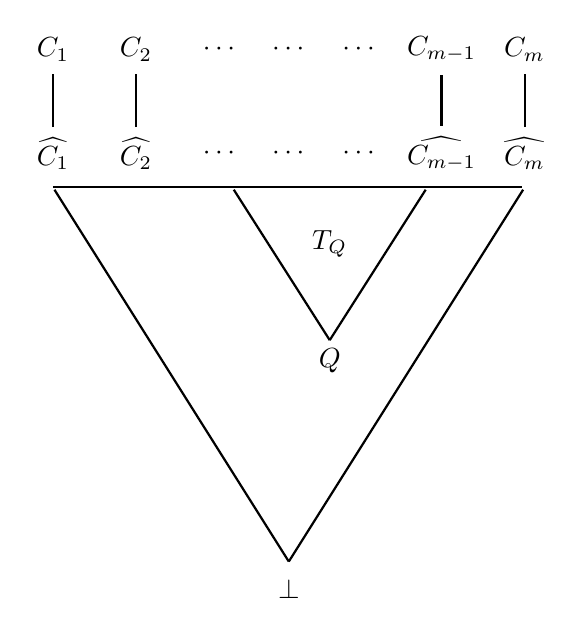
\begin{tikzpicture}[->,>=stealth,shorten >=1pt,auto,node distance=1.75cm, thick,main node/.style={scale=0.9,circle,draw,font=\sffamily\normalsize}]

        \node[] (2) []{};

        \node[] (2a) [above left of=2, xshift=-50, yshift=100]{};
        \node[] (2b) [above right of=2, xshift=50, yshift=100]{};
        \node[] (2c) [below of=2, yshift=40]{$\bot$};
        \node[] (2d) [above of=2]{};
        
        \node[] (3a) [right of=2a, xshift=15]{};
        \node[] (3) [below right of=3a, yshift=-20]{};
        \node[] (3b) [above right of=3, yshift=20]{};
        \node[] (3c) [above of=3, yshift=-15]{$T_Q$};
        \node[] (3c) [below of=3, yshift=42.5]{$Q$};


        \node[] (4) [above of = 2a, yshift = -37.5]{$\widehat{C_1}$};
        \node[] (5) [above of = 2a, yshift = -37.5, xshift=30]{$\widehat{C_2}$};
        \node[] (6) [above of = 2a, yshift = -37.5, xshift=60]{$\cdots$};
        \node[] (7) [above of = 2a, yshift = -37.5, xshift=85]{$\cdots$};
        \node[] (8) [above of = 2b, yshift = -37.5]{$\widehat{C_m}$};
        \node[] (9) [above of = 2b, yshift = -37.5, xshift=-30]{$\widehat{C_{m-1}}$};
        \node[] (10) [above of = 2b, yshift = -37.5, xshift=-60]{$\cdots$};


        \node[] (11) [above of = 2a]{${C_1}$};
        \node[] (12) [above of = 2a, xshift=30]{${C_2}$};
        \node[] (13) [above of = 2a, xshift=60]{$\cdots$};
        \node[] (14) [above of = 2a, xshift=85]{$\cdots$};
        \node[] (15) [above of = 2b]{${C_m}$};
        \node[] (16) [above of = 2b, xshift=-30]{${C_{m-1}}$};
        \node[] (17) [above of = 2b, xshift=-60]{$\cdots$};

        \path[every node/.style={font=\sffamily\small}, -]
            (4) edge (11)
            (5) edge (12)
            (8) edge (15)
            (9) edge (16)
            ;

        \path[every node/.style={font=\sffamily\small}, -]
            (2.center) edge (2a.center)
            (2.center) edge (2b.center)
            (2a.center) edge (2b.center)
            ;

        \path[every node/.style={font=\sffamily\small}, -]
            (3.center) edge (3a.center)
            (3.center) edge (3b.center)
            (3a.center) edge (3b.center)
            ;
    \end{tikzpicture}

    \caption{Representation of the idea behind \Cref{main_thm}}
\end{figure}

\quad

Again, thanks to \Cref{equiv_proof} and the fact that $\mathrm{PPA}^{dt}(S_F) = \Theta(\F_2\text{-}\mathsf{NS}(F))$, the last theorem proves that our new class is indeed contained inside $\mathsf{PPA}^{dt}$, meaning that any total search problem efficiently solvable by a parity decision tree can be reduced to an instance of the parity argument problem.  

\begin{theorem}
    $\mathsf{FP}^{pdt} \subseteq \mathsf{PPA}^{dt}$
\end{theorem}

\begin{proof}
 Suppose that $R \in \mathsf{FP}^{pdt}$. By definition, there is a PDT with size $s$ and depth $d$, where $d+\log s = O(\log^k n)$ for some $k \in \N$,that solves $R$. We know that each total search problem is equivalent to the false clause search problem of some CNF formula $F$, thus $R = S_F$.
    
 By \Cref{pdt_to_resp}, we know that there is a \textsf{TreeRes}$_{\oplus}$ proof of $F$ with size $O(s)$. Then, by theorem \Cref{main_thm}, we know that there must be a $\F_2$-Nullstellensatz refutation for $F$ with degree $O(\log(s) + w)$, where $w$ is the width of the proof. 
    
 Since $F$ has a $\F_2$-\textsf{NS} refutation of degree $O(\log s + w)$ and since $\mathsf{PPA}^{pdt} = \Theta(\F_2$-\textsf{NS}), by \Cref{equiv_proof} we know that there is an efficient reduction $S_F \leq_m \mathsf{PPA}^{dt}$, concluding that $R \in \mathsf{PPA}^{pdt}$

\end{proof}

\newpage



\cleardoublepage